\documentclass[12pt,a4paper]{report}
\usepackage[utf8]{inputenc}
\usepackage{amsmath}
\usepackage{amsfonts}
\usepackage{amssymb}
\usepackage{graphicx}
\usepackage{caption}
\usepackage{svg}
%\usepackage{gensymb}
\usepackage{fourier}
\usepackage[francais]{babel}

\usepackage{moreverb}
%\usepackage{multirow}
%\author{LEJEUNE Raphaël}
%\title{Titre}

\usepackage[fpms]{umons-coverpage}
\umonsAuthor{Raphaël \textsc{LEJEUNE} \\ Maximilien \textsc{POTTIEZ}}
\umonsTitle{Un robot contrôlé via un Raspberry Pi}
\umonsSubtitle{Projet d'informatique}
\umonsDocumentType{Rapport de projet}
\umonsSupervisor{Sous la direction de Monsieur le Professeur\\ Mohammed \textsc{BENJELLOUN}}
\umonsDate{2015}

\begin{document}

\umonsCoverPage

\tableofcontents

\chapter{Introduction}

Décrire le but visé, l'utilité du robot.

Faire en français et en anglais !

\begin{figure}[hf!]
\center
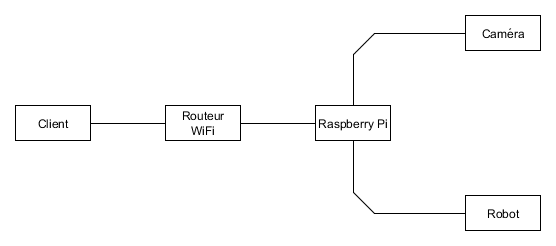
\includegraphics[scale=0.6]{GraphMateriel.png}
\caption{Matériel}
\end{figure}

\chapter{Matériel}

Lister le matériel utilisé, justifier sa présence

- Raspberry (pourquoi pas un Arduino, par exemple ?)
- Moteurs (quel modèle ?)
- Contrôleur (expliquer son utilité)
- Batterie
- Clé wifi
- Webcam (caractéristiques techniques)
- Réseau Wi-Fi opérationnel
- ?

\chapter{Software}

%Trouver un autre titre !!!

%Ici expliquer le principe des signaux PWM, des sockets, du multi-thread (même si pas utilisé... Parler des pistes envisagées)

%Captures d'écran

Lors de la réalisation du projet, nous avons envisagé plusieurs pistes pour contrôler le robot. 

\section{Signaux PWM}

Pour contrôler les moteurs, nous pouvons utiliser les signaux PWM (\textit{Pulse Width Modulation}) : il s'agit d'ondes carrées périodiques. 

Pour chaque période, on envoie une tension continue de 5 volts (qui correspond à la tension de base du Raspberry Pi, délivrée sur les ports GPIO) pendant une fraction de la période seulement. La tension « perçue » par le moteur est directement proportionnelle à cette fraction. Si cette fraction vaut par exemple 60 \%, le moteur tournera comme si on envoyait 3 V, donc à 60 \% de son régime maximum, si sa tension nominale est de 5 V. 

\chapter{Notre code}

\begin{figure}[hf!]
\center
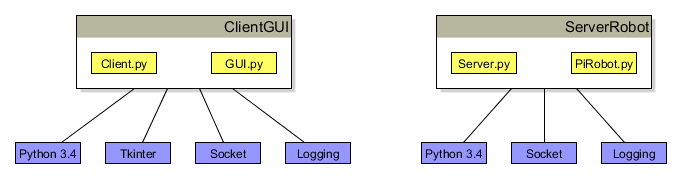
\includegraphics[scale=0.6]{GraphLogiciel.png}
\caption{Logiciel}
\end{figure}

Notre code est divisé en deux parties :

\bigbreak

\begin{itemize}
\item La partie client, qui tourne sur un PC (sous Windows, Linux, ...),
\item La partie serveur, qui se trouve sur le Raspberry Pi.
\end{itemize}

\bigbreak

\paragraph{Client.py}

Ce fichier sert à communiquer avec le Raspberry Pi. C'est dans ce fichier que sont récupérées toutes les requêtes de l'utilisateur, lorsqu'il appuie sur un bouton, par exemple.

\paragraph{GUI.py}

Ce fichier sert à tracer l'interface graphique. Nous avons voulu créer des fonctions dans ce fichier et les lier directement au bouton comme ci-après :

\begin{verbatimtab}[3]
buttonstop = Button(frameRoot, text="STOP", command=buttonstopclick)
\end{verbatimtab}

Mais cela a entraîné des erreurs de références circulaires (car \textit{Client.py} dépend de \textit{GUI.py} et \textit{GUI.py} dépend de \textit{Client.py}). Nous avons résolu ce problème en ne donnant pas de fonction au bouton. Dans \textit{Client.py}, nous donnons explicitement la commande suivante :

\begin{verbatimtab}[3]
GUI.buttonstop.bind("<Button-1>", buttonstopclick)
\end{verbatimtab}

Cette seconde option présente deux avantages : on peut choisir le type d'événement à associer (bouton cliqué ou relâché, ...), et on peut aussi supprimer ce lien (avec la commande \verb=unbind=).

\paragraph{Server.py}

C'est le programme qui tourne sur le Raspberry Pi. Son but est de recevoir les messages (depuis le client) et de les interpréter pour envoyer des instructions au robot.

\paragraph{PiRobot.py}

C'est une classe qui contient toutes les fonctions d'envoi de commandes au robot, ainsi quand \textit{Server.py} reçoit un message, il n'a qu'à appeler la bonne fonction (par exemple la fonction \verb=Stop=, qui envoie une commande au robot pour arrêter les moteurs).

\paragraph{Python 3.4}

Ça peut sembler anodin, mais certaines fonctionnalités que nous utilisons n'existent pas ou existent sous un autre nom dans des versions antérieures de python. C'est pourquoi il est important de préciser que le code est exécuté avec Python 3.4.

\paragraph{Tkinter}

Nous nous servons de \textit{Tkinter} pour tracer l'interface graphique. Il permet d'organiser assez facilement les éléments dans la fenêtre graphique.

\paragraph{Socket}

Comme son nom l'indique, \textit{Socket} permet d'ouvrir une connection entre une machine hôte (appelée Serveur) et une ou plusieurs machines (appelées Clients). Une fois la connection établie, les commandes \verb=send= et \verb=recv= permettent d'échanger des données.

\paragraph{Logging}

\textit{Logging} sert à générer un fichier \text{.log}, contenant diverses informations. A titre d'exemple, la commande suivante est appelée dans la fonction \verb=buttonstopclick= :

\begin{verbatimtab}[3]
logging.debug('Button STOP click')
\end{verbatimtab}

Dans le fichier \text{.log}, on verra cette ligne :

\begin{verbatimtab}[3]
2015-07-28 18:06:08,051 root	DEBUG	Button STOP click
\end{verbatimtab}

C'est une alternative au \verb=print('Button STOP click')=, et qui permet de sauvegarder les actions faites lors de l'exécution d'un programme, même s'il est arrêté pour quelque raison que ce soit.

\chapter{Qui a fait quoi}

Environ 1 page par étudiant, détailler ce qu'il a fait

\chapter{Conclusion}

Difficultés rencontrées, limitations, améliorations possibles, ...

\appendix
\chapter{1234}

Procédure d'installation ? Soit générer un exécutable, soit faire exécuter avec python 3.4 (pas 2.7)

En 2 parties : client et serveur, + configuration (adresse IP, ...)

Partie client : possibilité de donner l'image d'une machine virtuelle, correctement configurée

\end{document}

